\documentclass[11pt, a4paper]{article}
\setlength{\headheight}{17.74934pt}
\addtolength{\topmargin}{-5.74934pt}
\usepackage[spanish]{babel}
\usepackage[utf8]{inputenc}
\usepackage{enumitem}
\usepackage{tikz}
\usepackage{titling}
\usepackage{graphicx}
\usepackage{fancyhdr}
\usepackage{amsmath}
\usepackage{amssymb}
\usepackage{geometry}
\usepackage{multicol}
\usepackage{cancel}
\usepackage{pgfplots}
\usepackage{float}
\pgfplotsset{compat=1.18}
\setlength{\parskip}{1em}
\setlength{\parindent}{0pt}

\pagestyle{fancy}
\fancyhf{}
\fancyhead[L]{
\includegraphics[width=2cm]{assets/logo-utp.png}} % Reemplaza con la ruta de tu imagen
\fancyhead[R]{\textbf{Matemática Discreta}}

\fancyfoot[R]{\thepage} % Número de página alineado a la derecha

\setlength{\textheight}{23cm}  % Ajusta el alto del texto (puedes aumentar este valor)



\title{
  
\includegraphics[width=5cm]{./assets/logo-utp.png} \\
  \vspace{1cm}
  \textbf{Universidad Tecnológica del Perú} \\
  \vspace{3.5cm}
  \textbf{Exploración de Algoritmos de Búsqueda en el Marco de Estructuras Discretas: Un Estudio de Grafos y Árboles} \\ 
  \vspace{1cm}
  \large \textbf{Para el curso de Matemática Discreta}
}
  \author{\textbf{Luis Huatay S.}\\\\\texttt{hsluis4326@gmail.com}\\\\\texttt{U24218809 - 35096}}
  \vspace{-1cm}

\begin{document}
\newgeometry{top=4cm}
\maketitle
\begin{center}
Docente Mg. Mattos Quevedo, Juan Manuel
\end{center}
\restoregeometry

\newpage 

\tableofcontents

% \begin{enumerate}[label=\arabic*.]
%   \item Introducción
%   \item Objetivos
%   \begin{enumerate}[label=2.\arabic*]
%     \item Objetivo General
%     \item Objetivos Específicos
%   \end{enumerate}
%   \item Sobre los Algoritmos de Búsqueda
%   \begin{enumerate}[label=3.\arabic*]
%     \item ¿Qué son los Algoritmos de Búsqueda?
%     \item Tipos de Algoritmos de Búsqueda
%     \item Aplicaciones
%     \begin{enumerate}[label=3.3.\arabic*]
%       \item Grafos
%       \item Árboles
%     \end{enumerate}
%   \end{enumerate}
%   \item Sobre la Teoría de Grafos
%   \item Sobre la Teoría de Árboles
%   \item Referencias
% \end{enumerate}

\newpage
\vspace*{\fill}
\section{Introducción}

La matemática discreta es una rama de las matemáticas que se ocupa de estructuras que son fundamentalmente discretas en lugar de continuas (diferencias entre racionales y enteros). La matemática discreta es esencial para la informática y la ciencia de la computación, ya que proporciona las bases teóricas para diversas áreas, como la teoría de grafos, la teoría de conjuntos, la teoría de números y la combinatoria. En este informe, exploraremos la cómo la teoría de grafos y árboles se relacionan con los algoritmos de búsqueda y cómo se aplican en la práctica.

  
\vspace*{\fill}

\newpage

\section{Objetivos}

  Los objetivos de este informe son establecidos con el fin de explorar y comprender la relación entre los algoritmos de búsqueda y la teoría de gráfos y árboles, para lo cual se plantean los siguientes:

  \subsection{Objetivo General}

  Analizar y comprender la aplicación de algoritmos de búsqueda en el marco de estructuras discretas, con énfasis en la teoría de grafos y árboles.

  \subsection{Objetivos Específicos}

  \begin{enumerate}
    \item Describir los conceptos fundamentales de los algoritmos de búsqueda y su relación con la teoría de grafos y árboles.
    \item Explicar la diferencia entre algunos tipos de algoritmos de búsqueda.
    \item Describir sus aplicaciones en la resolución de problemas prácticos con especial enfoque en el uso de grafos y árboles.
    \item Describir las herramientas matemáticas y conceptos teóricos que sustentan los algoritmos de búsqueda en estructuras discretas.
  \end{enumerate}

  \newpage

  \section{Sobre los Algoritmos de Búsqueda}

  Los algoritmos de búsqueda son procedimientos computacionales que se utilizan para encontrar una solución a un problema específico. Estos algoritmos se aplican en una amplia variedad de campos, como la inteligencia artificial, la optimización, la informática y la ciencia de datos. Los algoritmos de búsqueda se basan en la exploración sistemática de un espacio de soluciones para encontrar la mejor solución posible. Existen diferentes tipos de algoritmos de búsqueda, cada uno con sus propias características y aplicaciones.

  Según Fernandez J. (2018) Cualquier algoritmo se define, de forma básica, como el conjunto ordenado y finito de operaciones que permite encontrar la solución de un problema [Real Academia Española, 2018]. Aplicando esta definición a los problemas tratados en este trabajo, un algoritmo de búsqueda se estructura como una secuencia de pasos, finita, que debe realizarse para alcanzar un objetivo establecido de antemano. Estos algoritmos se caracterizan por los siguientes aspectos:

  \begin{itemize}
    \item \textbf{Completitud:} Característica que aquellos algoritmos que son capaces de encontrar, al menos, una solución al problema, si es que existe alguna.
    \item \textbf{Admisibilidad:} Característica de los algoritmos que retornan como solución la óptima en caso de existir alguna. Este aspecto también es denominado optimalidad.
  \end{itemize}

  \begin{flushright}
    \textit{Fernandez, J. (2018). Cálculo de trayectos mediante algoritmos de búsqueda informada sobre grafos ponderados dirigidos.}
  \end{flushright}

  \subsection{¿Qué son los Algoritmos de Búsqueda?}

  Es entonces y de acuerdo a lo mencionado que podríamos definir a los algoritmos de búsqueda como aquellos procedimientos que permiten encontrar una solución a un problema específico, mediante la exploración sistemática de un espacio de soluciones. En consecuencia, los algoritmos de búsqueda son fundamentales en la resolución de problemas complejos, ya que permiten encontrar la mejor solución posible en un tiempo razonable.

  Hoy en día estas herramientas hacen posible la resolución de problemas en áreas como la inteligencia artificial, la optimización, la informática y la ciencia de datos, entre otras, inclusive en la vida cotidiana, como en la búsqueda de rutas óptimas en aplicaciones de mapas. De hecho, es en este último ejemplo donde podemos ver reflejado el concepto de grafo, ya que las calles y avenidas de una ciudad pueden ser representadas como nodos y aristas, respectivamente, en un grafo, lo que permite aplicar algoritmos de búsqueda para encontrar la ruta más corta entre dos puntos.

  \newpage 

  \subsection{Tipos de Algoritmos de Búsqueda}

  Existen diferentes tipos de algoritmos de búsqueda, cada uno con sus propias características y aplicaciones.
  Algunos de ellos pueden ayudar a encontrar la solución óptima, mientras que otros pueden encontrar una solución aceptable en un tiempo razonable. Algunos de los tipos de algoritmos de búsqueda más comunes son:

  \begin{enumerate}
    \item \textbf{Búsqueda en Profundidad:} Este algoritmo explora un camino hasta que no haya más nodos por explorar, luego retrocede y explora otro camino. Es útil para encontrar soluciones en árboles y grafos con profundidad limitada.
    \item \textbf{Búsqueda en Anchura:} Este algoritmo explora todos los nodos a una profundidad dada antes de pasar a la siguiente profundidad. Es útil para encontrar la solución más corta en grafos no ponderados.
    \item \textbf{Búsqueda A*:} Este algoritmo utiliza una función heurística para estimar el costo de llegar a la solución. Es útil para encontrar la solución óptima en grafos ponderados.
    \item \textbf{Búsqueda en Profundidad Iterativa:} Este algoritmo combina la búsqueda en profundidad y la búsqueda en anchura para encontrar la solución en grafos con profundidad desconocida.
    \item \textbf{Búsqueda Bidireccional:} Este algoritmo explora desde el nodo inicial y el nodo final al mismo tiempo, buscando un punto de encuentro. Es útil para encontrar la solución más corta en grafos grandes.
    \item \textbf{Búsqueda de Costo Uniforme:} Este algoritmo explora los nodos con el menor costo acumulado. Es útil para encontrar la solución óptima en grafos con costos no uniformes.
    \item \textbf{Búsqueda en Haz:} Este algoritmo explora múltiples caminos al mismo tiempo, manteniendo solo los mejores caminos. Es útil para encontrar la solución en grafos grandes con muchos nodos.
    \item \textbf{Búsqueda Tabú:} Este algoritmo evita explorar caminos que ya se han explorado anteriormente. Es útil para encontrar soluciones diferentes en grafos con ciclos.
    \item \textbf{Búsqueda Genética:} Este algoritmo utiliza conceptos de evolución y selección natural para encontrar la solución óptima. Es útil para encontrar soluciones en problemas de optimización.
    \item \textbf{Búsqueda Local:} Este algoritmo explora el vecindario de una solución actual para encontrar una solución mejor. Es útil para encontrar soluciones en problemas de optimización.
  \end{enumerate}

\newpage

\subsection{Aplicaciones}

Los algoritmos de búsqueda tienen una amplia variedad de aplicaciones en la resolución de problemas prácticos. Algunas de las aplicaciones más comunes incluyen la búsqueda de rutas óptimas en mapas, la planificación de horarios, la optimización de rutas de transporte, la resolución de problemas de optimización y la planificación de tareas. En particular, los algoritmos de búsqueda son fundamentales en la resolución de problemas en grafos y árboles, donde se utilizan para encontrar la mejor solución posible en un espacio de soluciones complejas.

\subsubsection{Grafos}

  Una aplicación muy interesante de los algoritmos de búsqueda que utilicen grafos es en la representación de mapas geográficos y/o temáticos.
  
  Según Basso B, Ivo R. Álvarez N. Marcelino F. (2013) Los mapas siempre han fascinado a los topologos en virtud de ciertas cualidades que poseen. Al colorear un mapa geográfico, se acostumbra a asignar diferentes colores a dos regiones que tienen una porción de frontera que le es común. Se ha encontrado empíricamente, que cualquier mapa independiente del número de regiones que contenga y cómo éstas estén situadas. La mayoría de los mapas geográficos pueden interpretarse como grafos en lo que los vértices son los puntos de confluencia de tres o más líneas y las aristas son las líneas delimitantes de cada territorio o zona.

  \begin{flushright}
    \textit{Basso B, Ivo R. Álvarez N. Marcelino F. (2013). Teoría de Grafos.}
  \end{flushright}

  Las iterrogantes que derivan de lo anterior se expresan cómo:

  \begin{itemize}
    \item ¿Cuál es la mínima cantidad de colores necesaria para colorearlo de forma que zonas con frontera común tengan colores diferentes?
    \item ¿Cómo deben ser los mapas que son coloreables con tan sólo 2 colores? ¿Y con 3 
    colores presentaría mayor dificultad?
  \end{itemize}

  Según teorema: \textit{\textbf{Un mapa es coloreable con dos colores si y sólo si su grafo asociado 
  tiene todos sus vértices con grado par y mayor o igual que dos. }}

  Utilizando notación lógico-matemática, se puede expresar como:

  \begin{align*}
    \forall v \in V(G) \quad \text{gr}(v) \geq 2 \quad \land \quad \text{gr}(v) \equiv 0 \quad (\text{mod} \quad 2)
  \end{align*}

  \newpage

  \textbf{Por consiguiente:} Si el mapa se colorea con dos colores los vértices de su grafo tienen grado par, pues 
  si hubiese un vértice con grado impar al menos una cara lindaría como mínimo con 
  dos caras más y, por lo tanto, Se precisarían tres colores. 

  Un ejemplo de un plano coloreable con dos colores es el tablero de ajedrez:

  \begin{figure}[H]
    \centering
    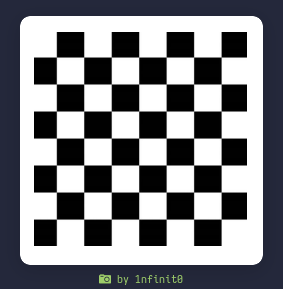
\includegraphics[width=5cm]{./assets/tablero_ajedrez.png}
    \caption{Tablero de Ajedrez}
    \label{fig:tablero-ajedrez}
  \end{figure}

  \textbf{Cuatro colores son suficientes:} Es fácil ver que un número menor de colores no es suficiente para todos los casos como lo muestran los siguientes diagramas:

  \begin{figure}[H]
    \centering
    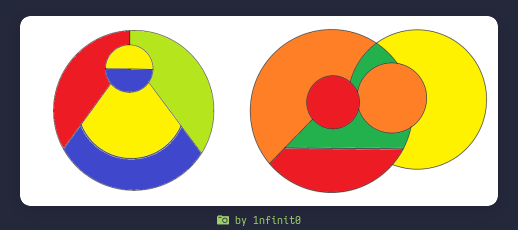
\includegraphics[width=10cm]{./assets/esfera_mapa.png}
    \caption{Región esférica coloreada}
    \label{fig:esfera-mapa}
  \end{figure}
  
  Las regiones no pueden colorearse con menos de cuatro colores ya que cada región tiene frontera con las otras tres. El caso de un mapa plano o uno esférico es lo mismo ya que cualquier mapa en una esfera puede transformarse en un mapa plano, agujereando la esfera y aplanándola. 

  El teorema de los cuatro colores, fue uno de los más famosos problemas no resueltos por la matemática. Fue planteado por primera vez en 1852. Kempe publicó una demostración en el año 1879, la cual contenía un error de razonamiento.

  Finalmente el problema de los cuatro colores fue resuelto por K. Appel y W. Haken en 1976. Su demostración, que les ocupó 4 años y una considerable cantidad de tiempo de computadoras. 

  
  \newpage

  \subsubsection{Árboles}

  Los algoritmos de búsqueda que fundamentan su funcionamiento en árboles son fundamentales en la resolución de problemas de optimización y planificación. Un ejemplo de aplicación de los algoritmos de búsqueda en árboles es la planificación de horarios en una universidad. Según Hinojosa E. (2014) Un Árbol binario de búsqueda, puede usarse como un Árbol de búsqueda binaria. Usando notación de Árbol Binario, el algoritmo para la búsqueda de la llave key en un Árbol de este tipo es como sigue (suponemos que cada nodo contiene cuatro campos: k, que guarda el valor de la llave del registro, r, que guarda el propio registro y left y right que son apuntadores a los sub Árboles).

  \begin{flushright}
    \textit{Hinojosa E. (2014). Velocidad de respuesta de los algoritmos de búsqueda en datos contenidos en estructuras dinánimas y estáticas.}
  \end{flushright}

  \textbf{Búsqueda de elementos de un árbol binarios (BST):} La búsqueda de un elemento en un árbol binario de búsqueda (BST) es un proceso que se realiza de forma recursiva. Se comienza comparando el elemento a buscar con la raíz del árbol. Si el elemento es igual a la raíz, se ha encontrado la solución. Si el elemento es menor que la raíz, se busca en el subárbol izquierdo. Si el elemento es mayor que la raíz, se busca en el subárbol derecho. Este proceso se repite hasta encontrar el elemento o llegar a un nodo nulo, en cuyo caso se concluye que el elemento no está en el árbol.

  Según el gráfico:

  \begin{figure}[H]
    \centering
    \begin{tikzpicture}
      \node {8}
        child {node {3}
          child {node {1}}
          child {node {6}
            child {node {4}}
            child {node {}}
          }
        }
        child {node {10}
          child[missing] {}
          child {node {14}
            child {node {?}}
            child[missing] {}
          }
        };
    \end{tikzpicture}
    \caption{Árbol Binario de Búsqueda}
    \label{fig:arbol-binario}
  \end{figure}


  \textbf{Algunas ventajas del uso de BST:}

  \begin{itemize}
    \item \textbf{Eficiencia:} La búsqueda en un árbol binario de búsqueda es eficiente, ya que el tiempo de búsqueda es proporcional a la altura del árbol.
    \item \textbf{Escalabilidad:} Los árboles binarios de búsqueda son escalables, lo que significa que pueden manejar grandes cantidades de datos de manera eficiente.
  \end{itemize}

\newpage

\section{Sobre la Teoría de Grafos}

  Son una herramienta matemática fundamental, que se utiliza para modelar y resolver problemas en una amplia variedad de campos, como la informática, la ingeniería, la biología y la economía. Un grafo es un conjunto de nodos (vértices) conectados por aristas (arcos), que se utilizan para representar relaciones entre entidades. Los grafos se utilizan para modelar una amplia variedad de problemas, como la planificación de rutas, la optimización de redes, la detección de comunidades y la resolución de problemas de flujo.

  Fue Euler quien en 1736, en su solución al problema de los siete puentes de Königsberg, introdujo la teoría de grafos. En este problema, Euler demostró que no era posible recorrer los siete puentes de la ciudad de Königsberg sin pasar dos veces por el mismo puente. Para ello, Euler representó los puentes y las tierras de Königsberg como nodos y aristas en un grafo, y demostró que el problema se podía resolver utilizando la teoría de grafos.

  Matemáticamente, un grafo se define como un par ordenado $G = (V, E)$, donde $V$ es un conjunto finito de nodos y $E$ es un conjunto de pares no ordenados de nodos que representan las aristas del grafo. Los grafos se pueden clasificar en diferentes tipos, como grafos dirigidos, grafos no dirigidos, grafos ponderados y grafos no ponderados, según las características de sus aristas.

\section{Sobre Árboles}

  Los árboles son una estructura de datos fundamental en informática y ciencias de la computación, que se utiliza para representar jerarquías y relaciones de dependencia entre entidades. Un árbol es un grafo acíclico dirigido, que consta de un conjunto de nodos (vértices) conectados por aristas (arcos) de tal manera que no forman ciclos. Los árboles se utilizan para modelar una amplia variedad de problemas, como la organización de archivos, la representación de estructuras de datos y la resolución de problemas de optimización.

  Fue Cayley quien en 1857, en su estudio de los árboles genealógicos, introdujo la teoría de árboles. En este estudio, Cayley demostró que el número de árboles con $n$ nodos es $n^{n-2}$, lo que se conoce como la fórmula de Cayley. Esta fórmula es fundamental en la teoría de árboles y se utiliza para contar el número de árboles posibles con un número dado de nodos.

\newpage

\begin{thebibliography}{9}
  \addcontentsline{toc}{section}{Referencias}

  \bibitem{Fernandez} 
  Fernandez, J. (2018). Cálculo de trayectos mediante algoritmos de búsqueda informada sobre grafos ponderados dirigidos.

  \bibitem{Basso} 
  Basso B, Ivo R. Álvarez N. Marcelino F. (2013). Teoría de Grafos.

  \bibitem{Hinojosa} 
  Hinojosa E. (2014). Velocidad de respuesta de los algoritmos de búsqueda en datos contenidos en estructuras dinánimas y estáticas.

\end{thebibliography}
\end{document}